掌握数据结构对开发者来说必不可少,大多数时候存储数据的方式决定了应用程序的效率。以电子邮件客户端为例,你可以设计一个电子邮件客户端,显示最近10封电子邮件,用户在使用你的应用两年内会收到数十万封电子邮件。当用户需要搜索电子邮件时,数据结构就会发挥重要作用。你储存成千上万封电子邮件的方式,排序和搜索它们的方法(算法)则非常重要。 \par
开发者在项目中努力寻找日常问题的最佳解决方案,使用经过验证的数据结构和算法可以极大地改善工作效率。好的程序最重要的特点是速度,我们可以通过设计新的算法,或使用现有的算法来得到良好的运行速度。 \par
最后,C++20引入了元类型的概念——描述其他类型的类型,这个强大特性使数据架构更加完整。 \par
C++标准模板库(STL)中包含了大量的数据结构和算法。我们将探索利用STL容器来使用数据结构有效地组织数据的方法,然后将深入研究STL提供的算法实现。理解和使用STL容器中的概念至关重要,因为C++20通过引入迭代器概念,对迭代器进行了重大改进。 \par
本章中,我们将了解以下内容: \par

\begin{itemize}
	\item 数据结构
	\item STL容器
	\item 概念和迭代器
	\item 主流算法
	\item 探索树和图
\end{itemize}

\noindent\textbf{}\ \par
\textbf{编译器要求} \ \par
g++编译器需要添加编译选项 \texttt{-std=c++2a} 来编译本章的代码。可以从这里获取本章的源码文件:https:/​/github.​com/PacktPublishing/Expert-CPP \par

\noindent\textbf{}\ \par
\textbf{数据结构} \ \par
开发者日可能很熟悉使用数组来存储和排序数据,也会在项目中大量使用数据结构,而不是数组。了解和应用正确的数据结构可能在程序性能中扮演着重要的角色。为了选择正确的数据结构,就需要更好地了解它们。一个明显的问题可能会出现:我们是否需要研究数据结构的集合——向量、链表、哈希表、图、树等。为了回答这个问题,让我们想象一个场景,在这个场景中,合适的数据结构的必要性将很明显地显现出来。 \par
介绍性内容中,我们提到了设计电子邮件客户端。让我们大致了解一下它的设计和实现。 \par
电子邮件客户端是列出不同发件人邮件的应用。我们可以在台式电脑或智能手机上安装它,或者使用浏览器版本。电子邮件客户端应用的主要任务包括发送和接收电子邮件。现在假设我们正在设计简单的电子邮件客户机,假设我们使用一些库来封装发送和接收电子邮件的工作,这让我们更专注于设计专门用于存储和检索电子邮件的机制。客户端用户能够查看驻留在收件箱的邮件列表,还应该考虑用户可能想要对电子邮件执行的操作。他们可以一个个的删除,或者一次性删除很多,也可以随机选择任何一封邮件,回复发件人或转发给其他人。 \par
我们将在第10章中讨论软件设计过程和最佳实践。现在,让我们构建一个简单的Email对象,如下所示: \par

\begin{lstlisting}[caption={}]
struct Email
{
	std::string subject;
	std::string body;
	std::string from;
	std::chrono::time_point datetime;
};
\end{lstlisting}

第一件困扰我们的事情是将一组电子邮件存储容易访问的结构中,数组听起来可能不错。假设我们将所有收到的电子邮件存储在一个数组中,如下面的代码块所示: \par

\begin{lstlisting}[caption={}]
// let's suppose a million emails is the max for anyone
const int MAX_EMAILS = 1'000'000;
Email inbox[MAX_EMAILS];
\end{lstlisting}

我们可以以任何形式存储10封电子邮件——这不会影响应用的性能。然而,随着时间的推移,电子邮件的数量会增长。对于新收到的电子邮件,将带有相应字段的Email对象推送到inbox数组中,数组的最后一个元素表示最近收到的电子邮件。因此,要显示最近10封电子邮件的列表,需要读取并返回数组的最后10个元素。 \par
当试图操作存储在inbox数组中的数千封电子邮件时,问题就出现了。如果想在所有的电子邮件中搜索“friend”这个词,就必须扫描数组中的所有电子邮件,并在单独的数组中收集包含单词friend的电子邮件: \par

\begin{lstlisting}[caption={}]
std::vector<Email> search(const std::string& word) {
	std::vector<Email> search_results;
	for (all-million-emails) {
		if (inbox[i].subject.contains(word)) {
			search_results.push_back(inbox[i]);
		}
	}
	return search_results;
}
\end{lstlisting}

对于小型集合来说,使用数组存储数据绰绰有余。处理更大数据集的应用中,这种情况会变得复杂。使用特定数据结构的目的是使应用运行得更流畅。前面的示例展示了一个简单的问题:搜索电子邮件列表以匹配特定的值。在电子邮件中进行查找时,需要在合理的时间范围内。 \par
如果假设电子邮件的主题可能包含最多10个单词,那么搜索电子邮件主题中的特定单词需要将该单词与主题中的所有单词进行比较。最坏的情况下,没有任何匹配。强调最坏的情况,是因为只有在这种情况下的查找,才需要检查主题中的每个单词。对成千上万的电子邮件执行同样的操作,会让用户等的不耐烦。 \par
就应用程序效率而言,为特定问题选择正确的数据结构至关重要,例如:假设使用哈希表将单词映射到Email对象,每个单词都将映射到包含该单词的电子邮件对象列表。这种方法将提高搜索操作的效率,如下图所示:\par

\begin{center}
	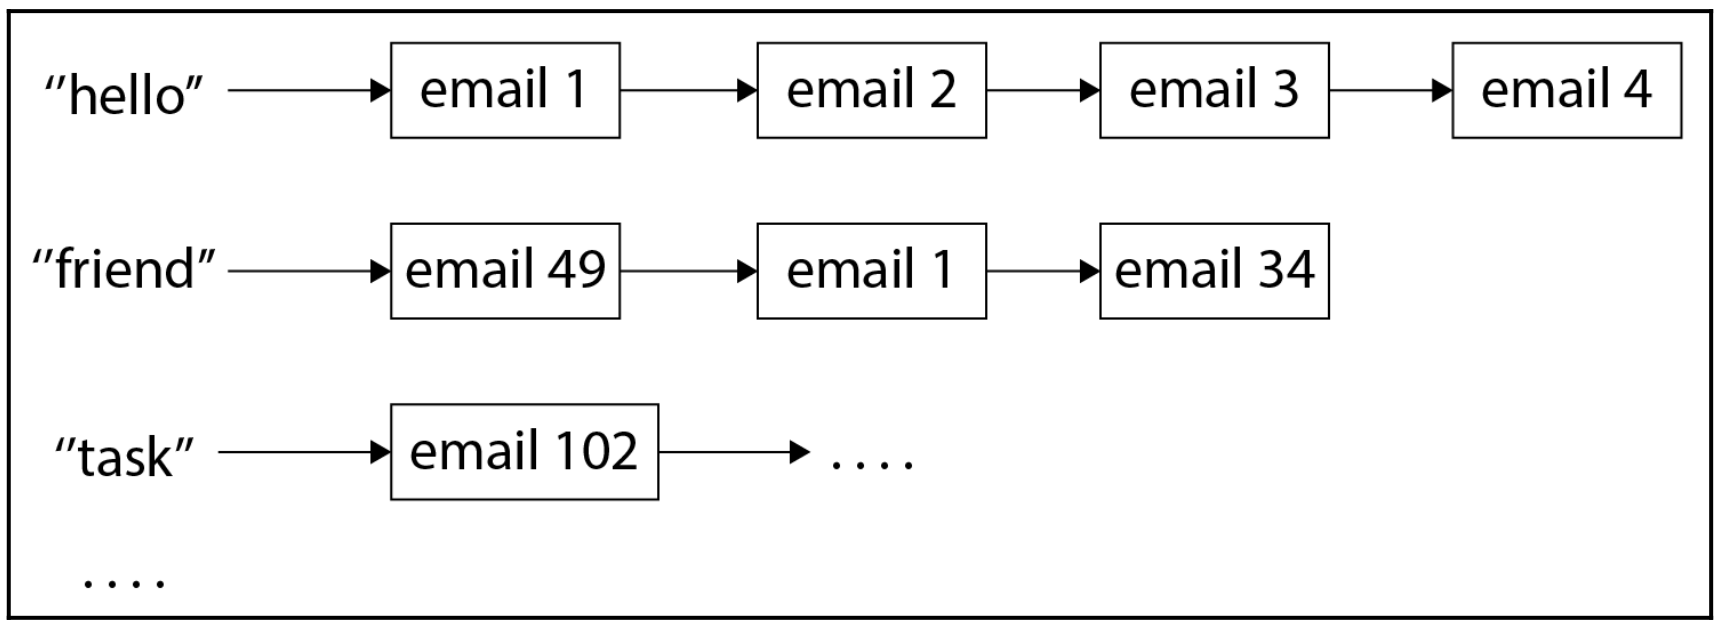
\includegraphics[width=0.6\textwidth]{content/Section-2/Chapter-6/1}
\end{center}

search()函数只返回哈希表键所指向的列表: \par

\begin{lstlisting}[caption={}]
std::vector<Email> search(const std::string& word) {
	return table[word];
}
\end{lstlisting}

这种方法只需要处理每个收到的电子邮件,将其拆分为单词并更新哈希表。 \par

\hspace*{\fill} \\ %插入空行

\includegraphics[width=0.05\textwidth]{images/tip}
简单起见,直接使用Email对象,而不是引用。请注意,最好将指向电子邮件的指针存储在vector中。 \par
\noindent\textbf{}\ \par

现在,让我们看看不同的数据结构及其应用。 \par

\noindent\textbf{}\ \par
\textbf{连续的数据结构} \ \par
开发人员使用的最常见数据结构是动态增长的一维数组——vector。STL提供了一个相同名称的容器:std::vector。vector的关键思想是,包含按顺序放置在内存中的相同类型的项。例如,由4个字节整数组成的向量,将具有如下的内存布局。每个框代表一个4字节的空间。向量的下标在下图的右侧: \par

\begin{center}
	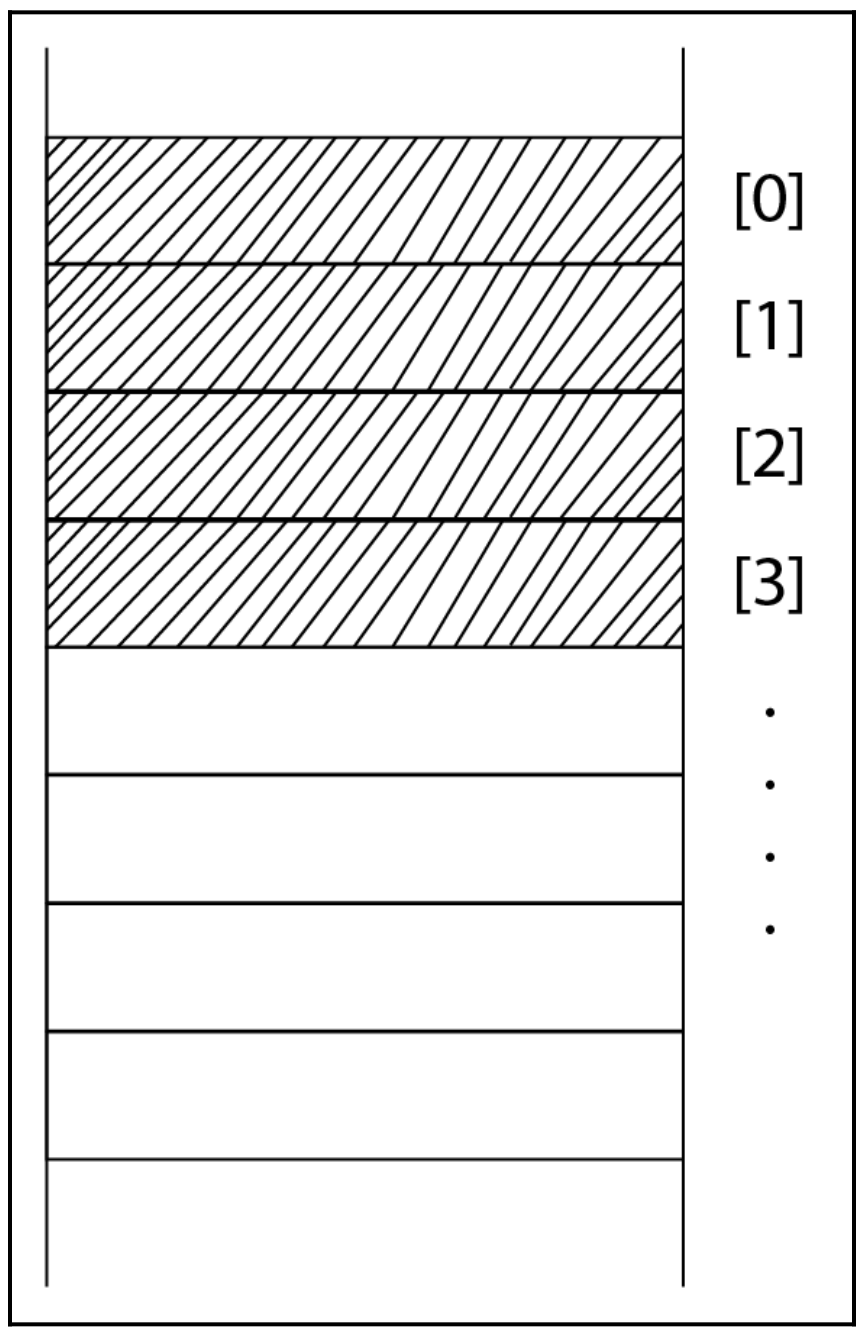
\includegraphics[width=0.4\textwidth]{content/Section-2/Chapter-6/2}
\end{center}

vector的物理结构允许实时访问它的任何元素。 \par

\hspace*{\fill} \\ %插入空行

\includegraphics[width=0.05\textwidth]{images/warn}
我们应该区分容器和操作,以便在问题中正确地应用。为此,我们根据容器中元素的数量定义操作时间复杂度。例如,vector的元素访问可定义为常量时间操作,这意味着无论vector的长度如何,访问vector中的项都需要相同数量的指令。 \par
\noindent\textbf{}\ \par

访问vector的第一个元素和访问向量的第100个元素需要相同的工作量,这就称之为常数时间操作,也称为O(1)操作。 \par

虽然vector中的元素访问速度很快,但添加新元素有点棘手。当在vector的末尾插入一个新元素时,还应该考虑vector的容量。当没有更多的空间分配给vector时,它应该动态地增加大小。看看下面的Vector类及其push\underline{ }back()函数: \par

\begin{lstlisting}[caption={}]
template <typename T>
class Vector
{
public:
	Vector() : buffer_{nullptr}, capacity_{2}, size_{0}
	{
		buffer_ = new T[capacity_]; // initializing an empty array
	}
	~Vector() { delete [] buffer_; }
	// code omitted for brevity
public:
	void push_back(const T& item)
	{
		if (size_ == capacity_) {
			// resize
		}
		buffer_[size_++] = item;
	}
	// code omitted for brevity
};
\end{lstlisting}

深入研究push\underline{ }back()函数的实现之前,让我们先看看下图: \par

\begin{center}
	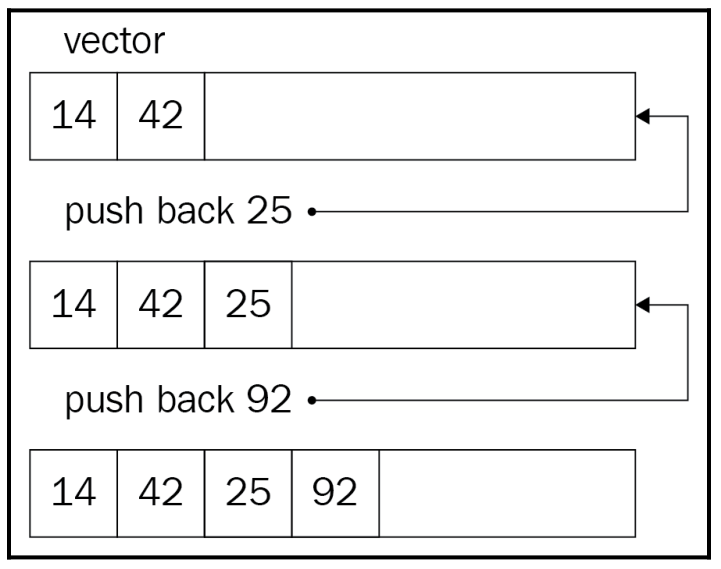
\includegraphics[width=0.6\textwidth]{content/Section-2/Chapter-6/3}
\end{center}

我们应该分配一个全新的数组,将旧数组的所有元素复制到新数组中,然后将新插入的元素添加到新数组末尾的下一个空闲槽中。如下面的代码片段所示: \par

\begin{lstlisting}[caption={}]
template <typename T>
class Vector
{
	public:
	// code omitted for brevity
	void push_back(const T& item)
	{
		if (size_ == capacity_) {
			capacity_ *= 2; // increase the capacity of the vector twice
			T* temp_buffer = new T[capacity_];
			// copy elements of the old into the new
			for (int ix = 0; ix < size_; ++ix) {
				temp_buffer[ix] = buffer_[ix];
			}
			delete [] buffer_; // free the old array
			buffer_ = temp_buffer; // point the buffer_ to the new array
		}
		buffer_[size_++] = item;
	}
	// code omitted for brevity
};
\end{lstlisting}

大小调整因子可以用不同的方式选择——我们将其设置为2,这将使vector在满载时,空间增长两倍。因此,我们坚持认为,大多数情况下,在向量的末尾插入一个新项需要常数时间。它只是在空闲槽添加项,并增加其私有size\underline{ }变量。有时,添加新元素需要分配一个新的、更大的vector,并需要将旧的vector复制到新的vector中。对于这样的情况,操作需要平摊常数时间才能完成。 \par
但当我们在vector前面加一个元素时就不能这么说了,所有其他元素都应该向右移动一个槽,以便为新元素腾出一个槽,如下图所示: \par

\begin{center}
	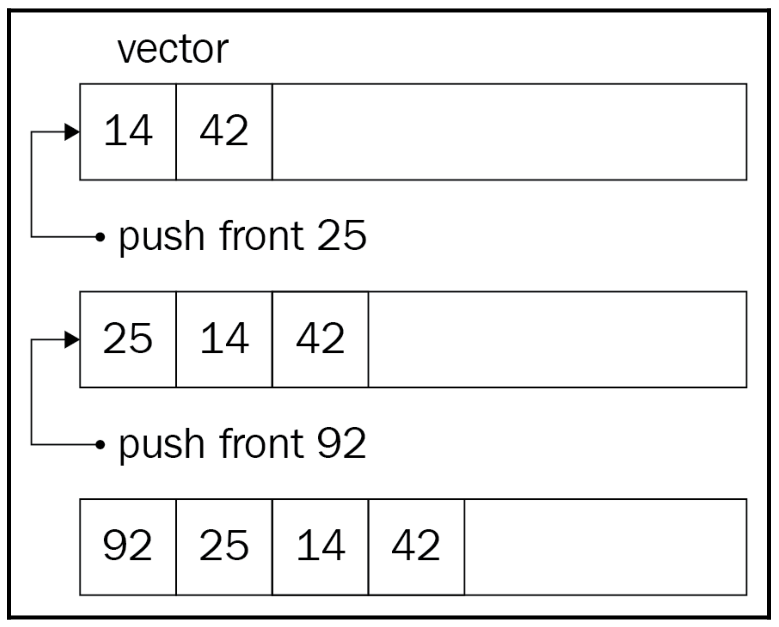
\includegraphics[width=0.6\textwidth]{content/Section-2/Chapter-6/4}
\end{center}

下面是我们如何在Vector类中实现它: \par

\begin{lstlisting}[caption={}]
// code omitted for brevity
void push_front(const T& item)
{
	if (size_ == capacity_) {
		// resizing code omitted for brevity
	}
	// shifting all the elements to the right
	for (int ix = size_ - 1; ix > 0; --ix) {
		buffer_[ix] = buffer[ix - 1];
	}
	// adding item at the front
	buffer_[0] = item;
	size_++;
}
\end{lstlisting}

在只需要在容器前端插入新元素的情况下,选择vector不是一个好的选择,这时需要考虑一下其他容器。 \par

\noindent\textbf{}\ \par
\textbf{节点式数据结构} \ \par
节点式的数据结构不需要连续的内存块。基于节点的数据结构为其元素分配节点,没有任何顺序——在内存中随机分布。我们将每个项目表示为一个节点,然后链接到其他节点的节点。 \par
最流行的、入门级的节点式的数据结构是链表。下面的图表可视化显示了双链表的结构: \par

\begin{center}
	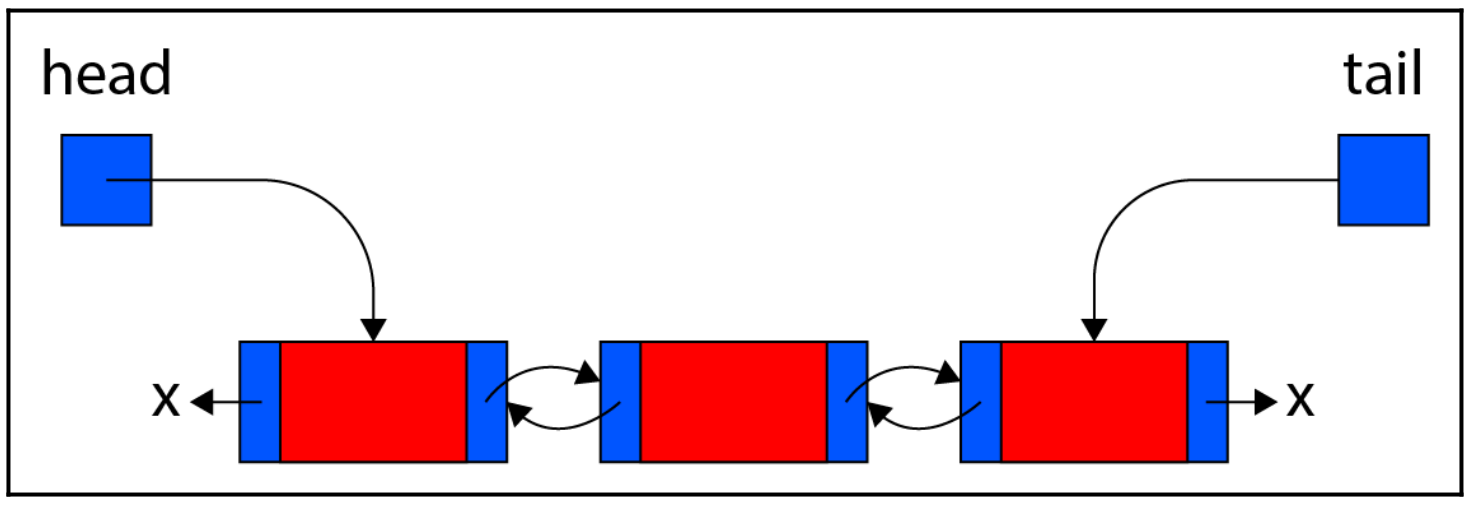
\includegraphics[width=0.6\textwidth]{content/Section-2/Chapter-6/5}
\end{center}

链表与向量有很大的不同。它的操作更快,但缺乏向量的紧凑性。 \par
为了保持简短,我们在列表的前面实现元素插入,将每个节点保持为一个结构体: \par

\begin{lstlisting}[caption={}]
template <typename T>
struct node
{
	node(const T& it) : item{it}, next{nullptr}, prev{nullptr} {}
	T item;
	node<T>* next;
	node<T>* prev;
};
\end{lstlisting}

请注意next成员——它指向同一个结构体,这种方式允许将节点链接在一起,如前面的示例所示。 \par
为了实现一个链表,需要一个指向它的第一个节点的指针,通常称为链表的头节点。在列表的前面插入一个元素很简单: \par

\begin{lstlisting}[caption={}]
template <typename T>
class LinkedList
{
	// code omitted for brevity
public:
	void push_front(const T& item)
	{
		node<T>* new_node = new node<T>{item};
		if (head_ != nullptr) {
			new_node->next = head_->next;
			if (head_->next != nullptr) {
				head_->next->prev = new_node;
			}
		}
		new_node->next = head_;
		head_ = new_node;
	}
private:
	node<T>* head_;
};
\end{lstlisting}

向列表中插入元素时,需要考虑以下三种情况: \par

\begin{itemize}
	\item 如前所述,在列表前面插入元素需要执行以下步骤: \par
	\begin{center}
		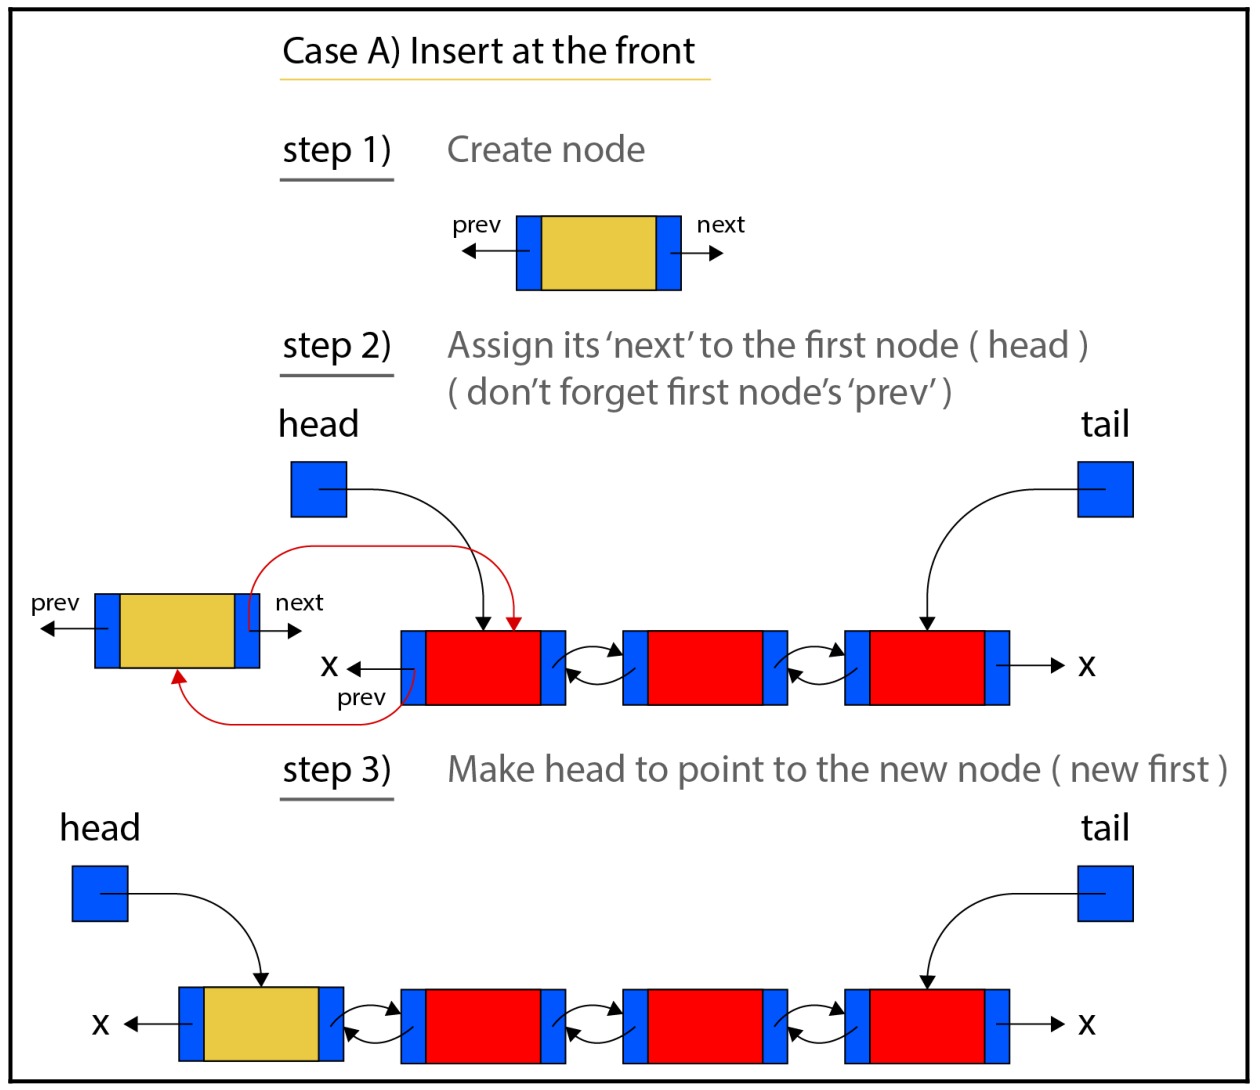
\includegraphics[width=0.6\textwidth]{content/Section-2/Chapter-6/6}
	\end{center}
	\item 在列表末尾插入一个元素,如下图所示: \par
	\begin{center}
		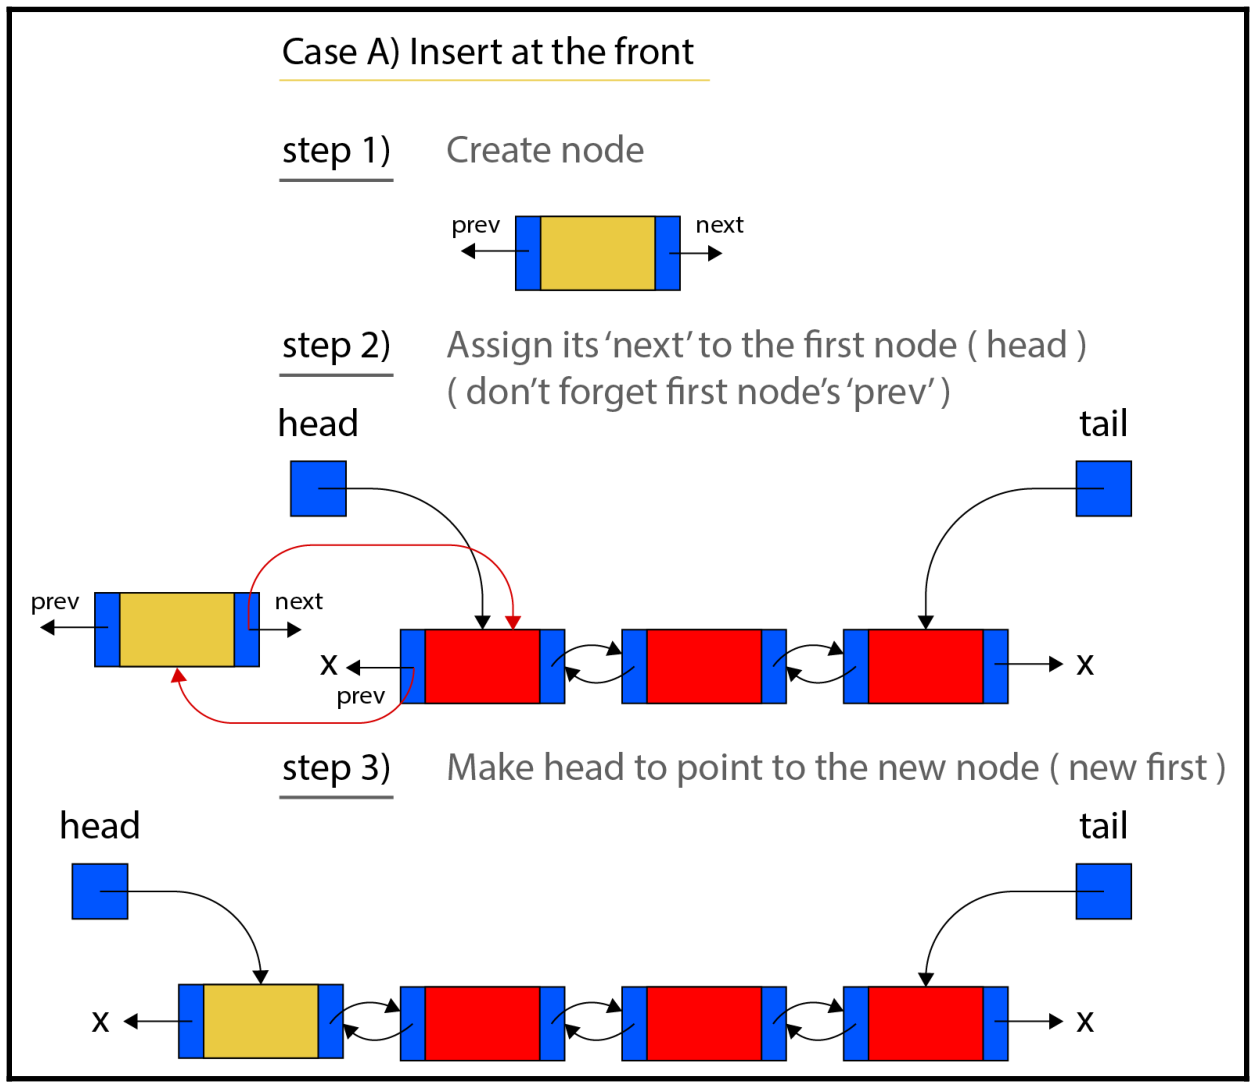
\includegraphics[width=0.6\textwidth]{content/Section-2/Chapter-6/7}
	\end{center}
	\item 最后,在列表中间插入一个元素的操作如下: \par
	\begin{center}
		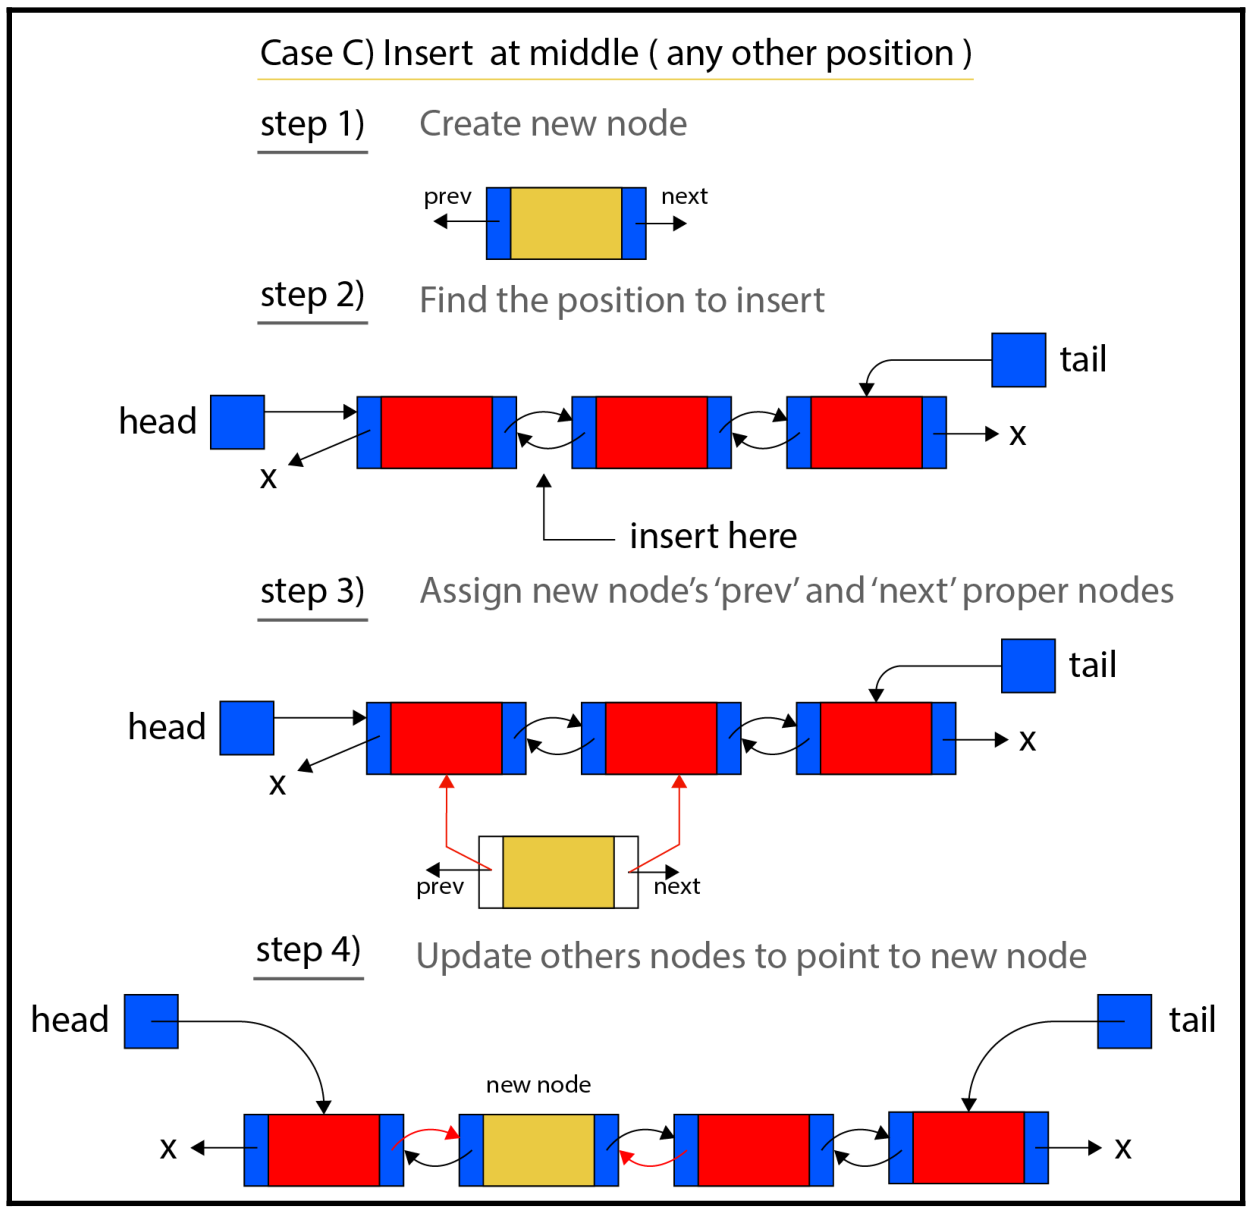
\includegraphics[width=0.6\textwidth]{content/Section-2/Chapter-6/8}
	\end{center}
\end{itemize}

向vector对象中插入元素与向list对象中插入元素明显不同。如何在vector和list中选择?应该专注行为和速度。例如,从vector中读取任何元素需要常量时间。我们可以在一个向量中存储100万封电子邮件,并且不需要任何额外的努力就可以检索位置为834,000的电子邮件。对于链表,操作是线性的。因此,如果需要存储主要用于读取而不是写入的数据集合,那么使用vector显然是合理的选择。 \par
在列表的任何位置插入元素需要常量时间的操作,而vector将努力在随机位置插入元素。因此,当需要一个可以集中添加/删除数据的对象集合时,更好的选择是一个链表。 \par
我们还应该考虑缓存内存。向量具有良好的数据局部性,读取vector对象的第一个元素需要将前N个元素复制到缓存中。进一步读取vector元素会更快。对于链表,我们就不能这么说了。为了找出原因,让我们继续比较vector和链表的内存布局。 \par

\noindent\textbf{}\ \par
\textbf{容器的内存} \ \par
如前面的章节所示,对象会在进程的内存段上占用一定的内存空间。大多数时候,我们感兴趣的是堆栈或堆内存。自动对象占用堆栈空间,下面两个声明都在栈中: \par

\begin{lstlisting}[caption={}]
struct Email
{
	// code omitted for brevity
};
int main() {
	Email obj;
	Email* ptr;
}
\end{lstlisting}

虽然ptr表示指向Email对象的指针,但也在堆栈上占用空间。可以指向在堆上分配的内存位置,但指针本身(存储内存位置地址的变量)驻留在堆栈上。进一步使用向量和列表之前,理解和记住这一点非常重要。 \par
如本章前面所示,实现vector涉及到封装指向内部缓冲区的指针,该缓冲区代表指定类型的元素数组。声明Vector对象时,需要一定数量的堆栈内存来存储其成员数据。Vector类有以下三个成员: \par

\begin{lstlisting}[caption={}]
template <typename T>
class Vector
{
public:
	// code omitted for brevity
private:
	int capacity_;
	int size_;
	T* buffer_;
};
\end{lstlisting}

假设一个整数占用4个字节,一个指针占用8个字节,下面的Vector对象声明将占用至少16个字节的堆栈内存: \par

\begin{lstlisting}[caption={}]
int main()
{
	Vector<int> v;
}
\end{lstlisting}

下面是我们对前面代码的内存布局的描述: \par

\begin{center}
	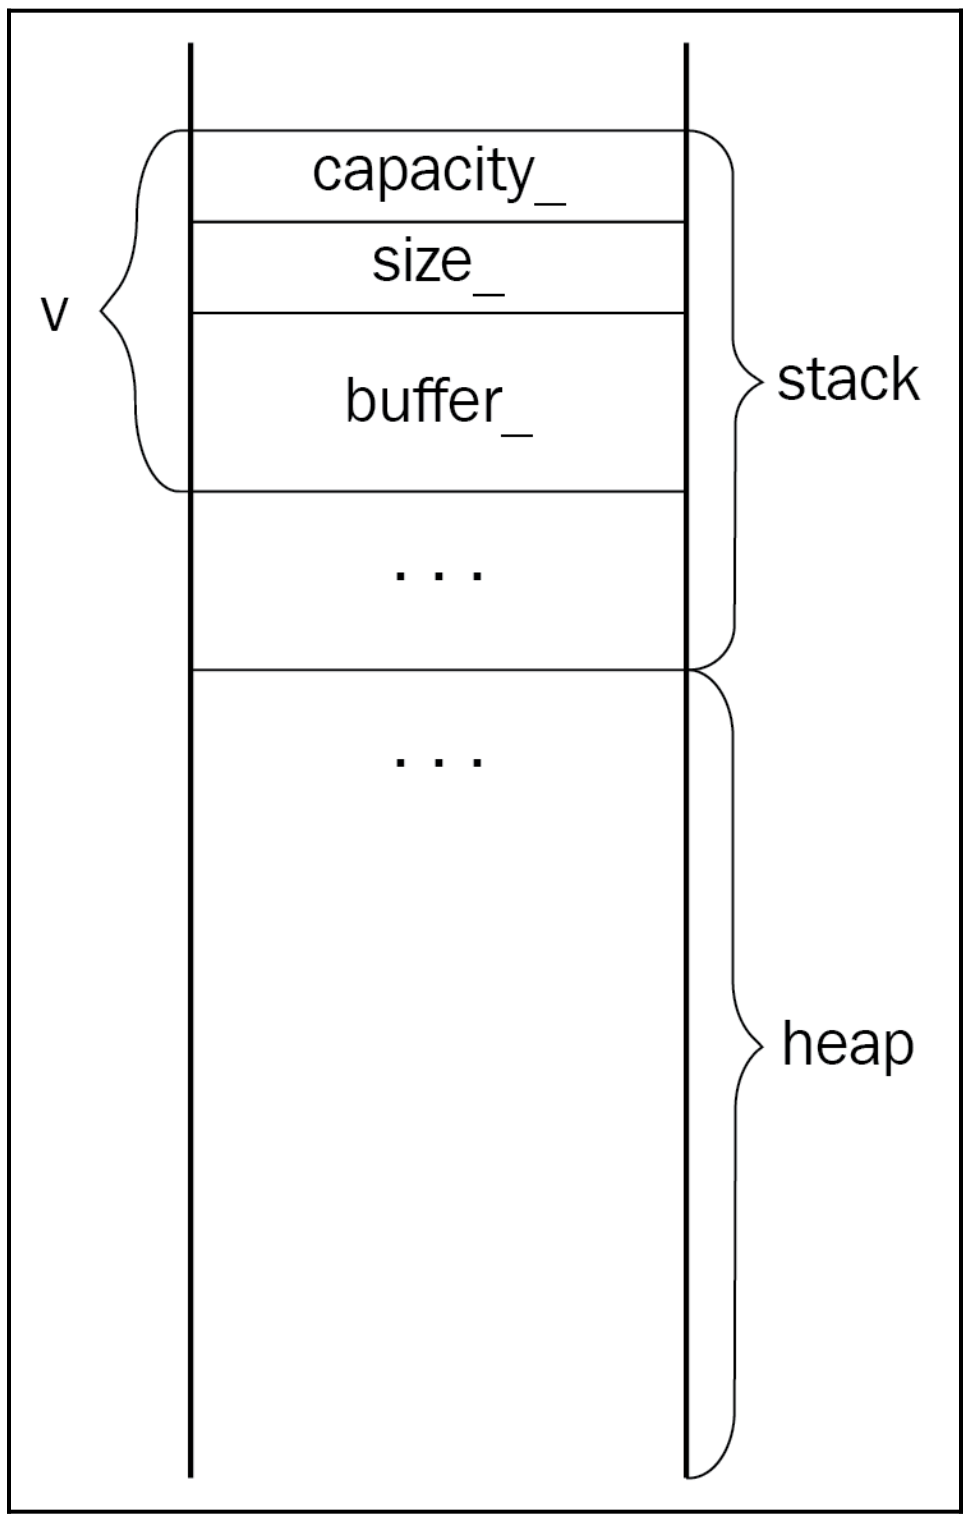
\includegraphics[width=0.4\textwidth]{content/Section-2/Chapter-6/9}
\end{center}

插入元素之后,堆栈上的vector对象的大小将保持不变,堆来保存现场。buffer\underline{ }数组指向一个使用new[]操作符分配的内存位置。例如下面的代码: \par

\begin{lstlisting}[caption={}]
// we continue the code from previous listing
v.push_back(17);
v.push_back(21);
v.push_back(74);
\end{lstlisting}

每一个推入vector的新元素都将占用堆中的空间,如下图所示: \par

\begin{center}
	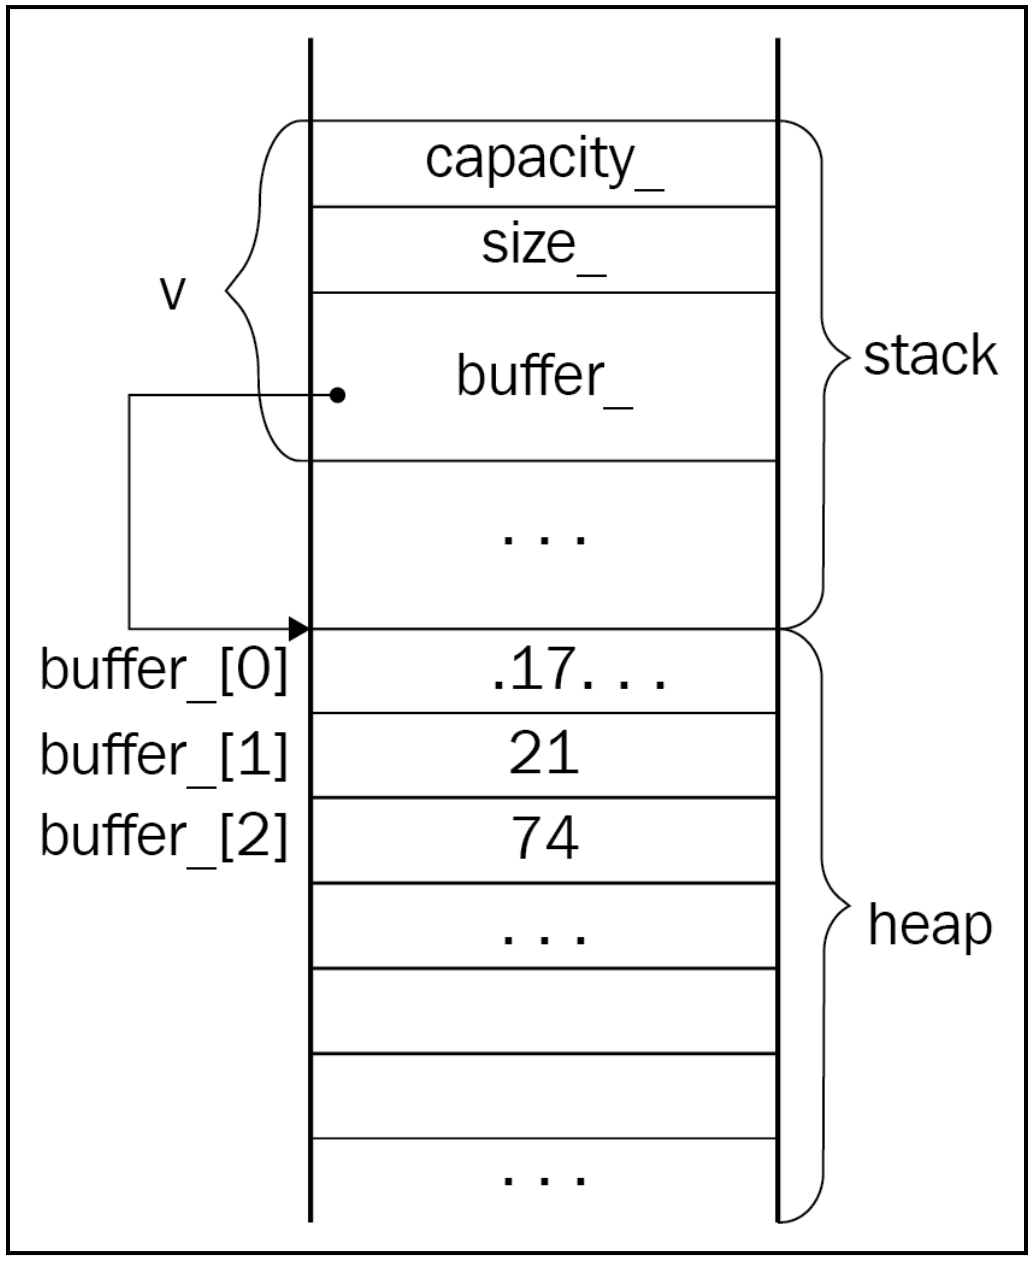
\includegraphics[width=0.6\textwidth]{content/Section-2/Chapter-6/10}
\end{center}

每个新插入的元素都位于buffer\underline{ }数组的最后。这就是为什么我们可以说vector是一个对缓存友好的容器。 \par
声明一个链表对象也会在堆栈上,为其数据成员占用内存空间。如果讨论只存储head\underline{ }指针的简单实现,那么下面的list对象声明将占用至少8个字节的内存(仅针对head\underline{ }指针): \par

\begin{lstlisting}[caption={}]
int main()
{
	LinkedList<int> list;
}
\end{lstlisting}

下面的图描述了上述代码的内存布局: \par

\begin{center}
	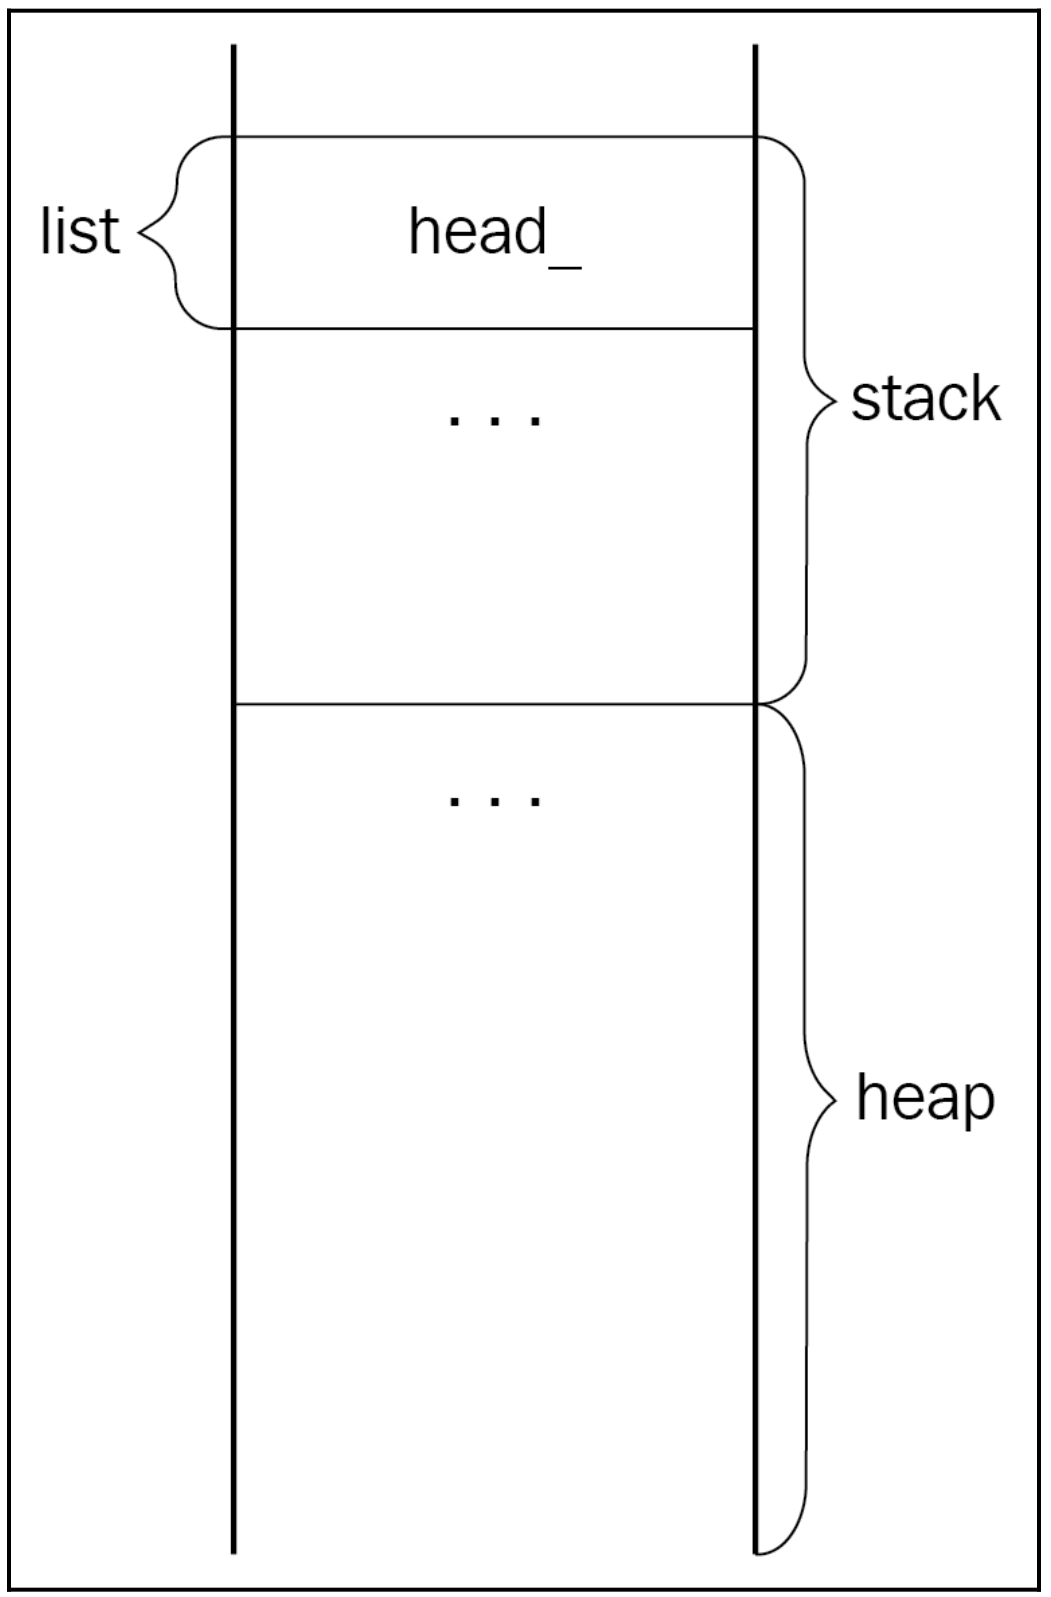
\includegraphics[width=0.4\textwidth]{content/Section-2/Chapter-6/11}
\end{center}

插入新元素会在堆上创建一个node类型的对象。看看下面这行: \par

\begin{lstlisting}[caption={}]
list.push_back(19);
\end{lstlisting}

下面是插入新元素后内存图的变化: \par

\begin{center}
	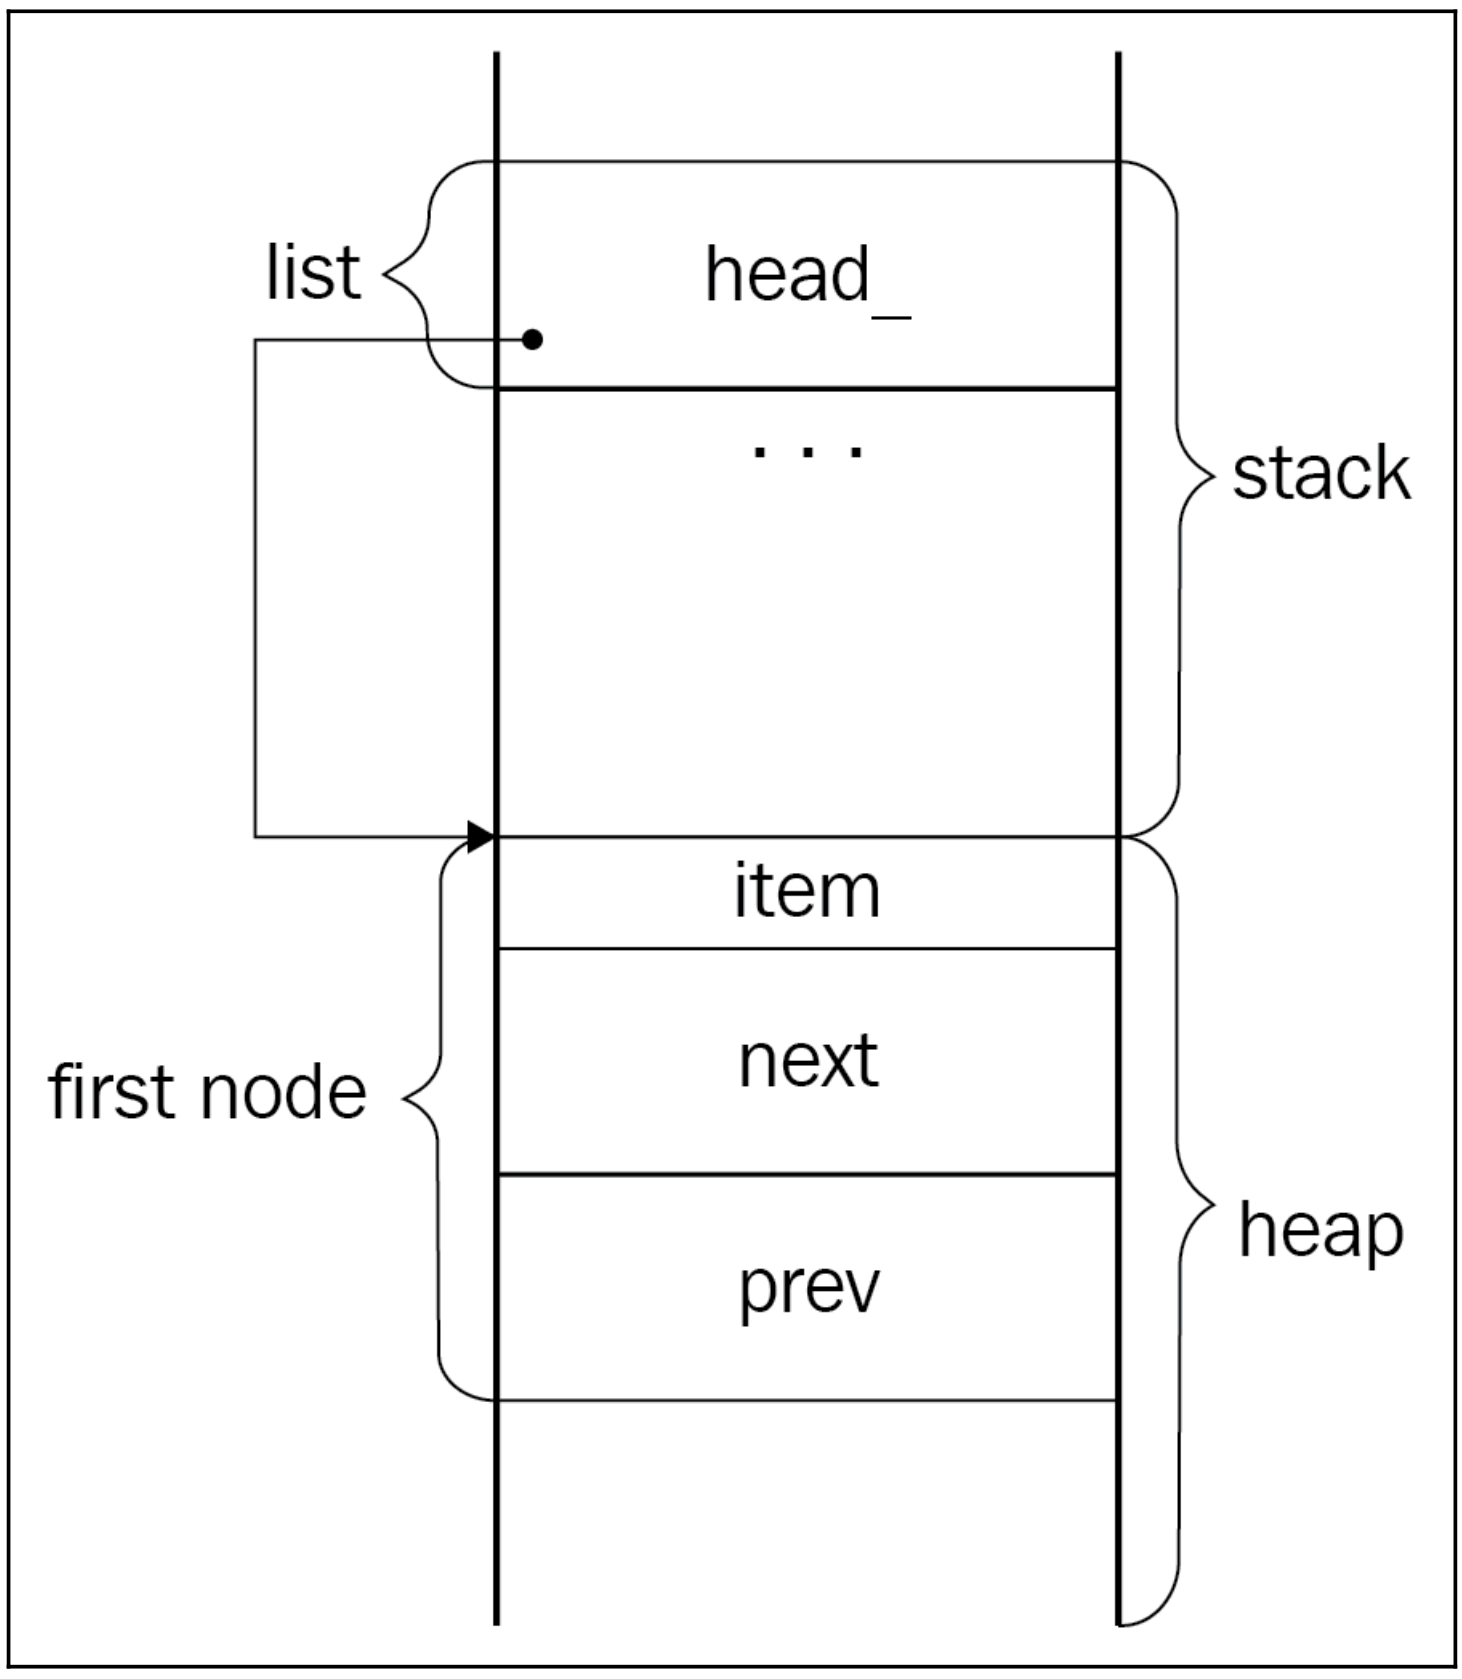
\includegraphics[width=0.6\textwidth]{content/Section-2/Chapter-6/12}
\end{center}

注意,节点的所有数据成员都驻留在堆上,item存储我们要插入的值。当我们插入另一个元素时,将再次创建一个新节点。这次,第一个节点的下一个指针将指向新插入的元素。新插入节点的prev指针将指向列表的前一个节点。下图描述了插入第二个元素后链表的内存布局: \par

\begin{center}
	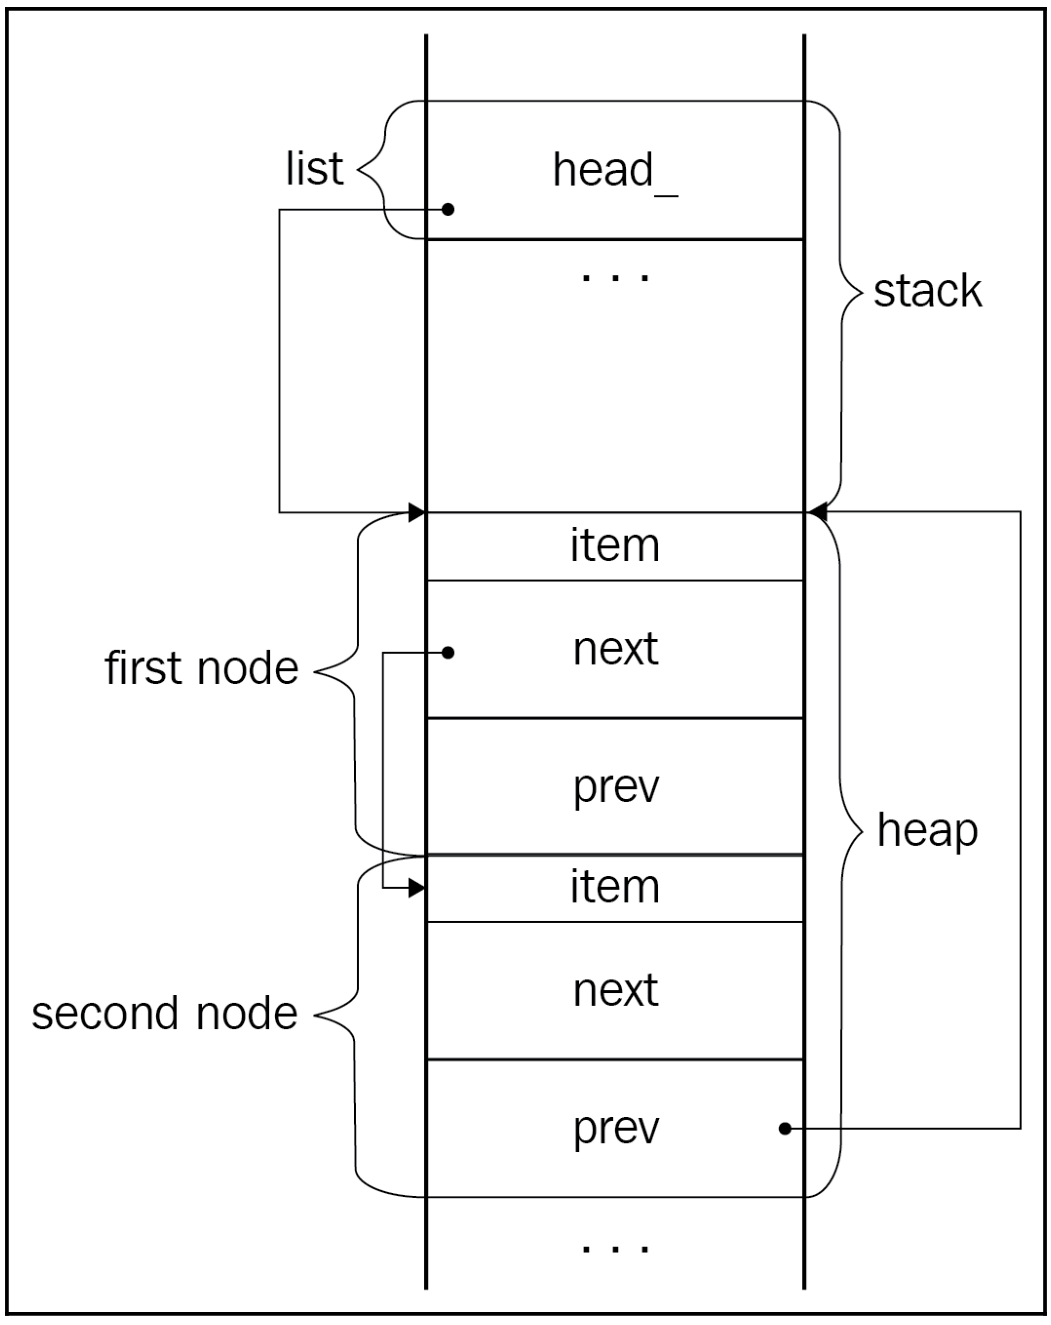
\includegraphics[width=0.6\textwidth]{content/Section-2/Chapter-6/13}
\end{center}

当向列表中插入元素的过程中在堆上分配一些随机对象时,会发生有趣的事情。例如,下面的代码将一个节点插入到列表中,然后为一个整数(与列表无关)分配空间。最后,再次向列表中插入一个元素: \par

\begin{lstlisting}[caption={}]
int main()
{
	LinkedList<int> list;
	list.push_back(19);
	int* random = new int(129);
	list.push_back(22);
}
\end{lstlisting}

这种中间随机对象声明破坏了列表元素的顺序,如下图所示: \par

\begin{center}
	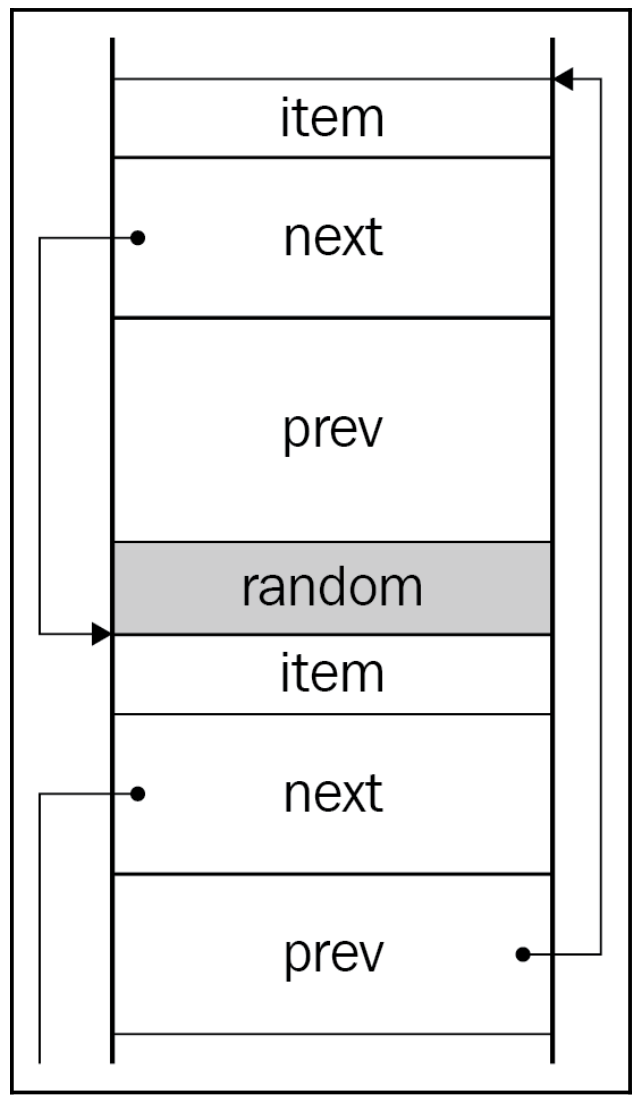
\includegraphics[width=0.4\textwidth]{content/Section-2/Chapter-6/14}
\end{center}

上面的图提示我们,由于列表的结构和元素的分配,它不是一个缓存友好的容器。 \par

\hspace*{\fill} \\ %插入空行

\includegraphics[width=0.05\textwidth]{images/tip}
请注意将每个新节点合并到代码中所产生的内存开销,我们为一个元素额外支付16个字节(考虑到指针需要8个字节的内存)。因此,在最佳内存使用的比拼中,列表输给了vector。 \par
\noindent\textbf{}\ \par

我们可以通过在列表中引入一个预先分配的缓冲区来解决这个问题。然后,每个新节点的创建都将通过重新实现的new操作符传递。更明智的做法是选择更适合问题的数据结构。 \par
实际的应用程序开发中,开发者很少自己实现向量或链表,通常会使用经过测试的稳定库版本。C++同时提供了vector和链表的标准容器。此外,为单链表和双链表提供了独立的两个容器。 \par

\noindent\textbf{}\ \par
\textbf{STL容器} \ \par

\noindent\textbf{}\ \par
\textbf{使用std::vector和std::list} \ \par

\noindent\textbf{}\ \par
\textbf{使用容器适配器} \ \par

\noindent\textbf{}\ \par
\textbf{迭代容器} \ \par

\noindent\textbf{}\ \par
\textbf{概念和迭代器} \ \par

\noindent\textbf{}\ \par
\textbf{理解概念} \ \par

\noindent\textbf{}\ \par
\textbf{在C++20中使用迭代器} \ \par

\noindent\textbf{}\ \par
\textbf{主流算法} \ \par

\noindent\textbf{}\ \par
\textbf{搜索} \ \par

\noindent\textbf{}\ \par
\textbf{二分搜索} \ \par

\noindent\textbf{}\ \par
\textbf{排序} \ \par

\noindent\textbf{}\ \par
\textbf{搜索树和图} \ \par

\noindent\textbf{}\ \par
\textbf{哈希表} \ \par

\noindent\textbf{}\ \par
\textbf{图} \ \par

\noindent\textbf{}\ \par
\textbf{字符串} \ \par

\noindent\textbf{}\ \par
\textbf{总结} \ \par

\noindent\textbf{}\ \par
\textbf{问题} \ \par
\begin{enumerate}
	\item 描述将元素插入动态增长向量的过程。
	\item 在链表的前面插入元素和在vector的前面插入元素有什么区别?
	\item 实现一个混合数据结构,将其元素存储在vector和list中。对于每个操作,选择具有最快实现该操作的底层数据结构。
	\item 如果我们按递增顺序插入100个元素,那么二叉搜索树会是什么样子呢?
	\item 选择排序和插入排序算法有什么区别?
	\item 实现本章中描述的排序算法,称为计数排序。
\end{enumerate}

\noindent\textbf{}\ \par
\textbf{扩展阅读} \ \par
有关更多信息,请参阅以下参考资料: \par

\begin{itemize}
	\item Programming Pearls by Jon Bentley, available from  https:/​/​www.​amazon.​com/	Programming-​Pearls-​2nd-​Jon-​Bentley/​dp/​0201657880/​
	\item Data Abstraction and Problem Solving Using C++: Walls and Mirrors by Frank Carrano,and Timothy Henry, available from  https:/​/​www.​amazon.​com/​Data-Abstraction-​Problem-​Solving-​Mirrors/​dp/​0134463978/​
	\item Introduction to Algorithms by Cormen, Leiserson, Rivest, and Stein, available
	from https:/​/​www.​amazon.​com/​Introduction-​Algorithms-​3rd-​MIT-​Press/​dp/0262033844/​
	\item C++ Data Structures and Algorithms by Wisnu Anggoro, available from  https:/​/
	www.​packtpub.​com/​application-​development/​c-​data-​structures-​and-algorithms
\end{itemize}

\newpage







